\documentclass{article}
\usepackage{icmcsmc2014}
\usepackage{times}
\usepackage{ifpdf}
\usepackage[english]{babel}
%\usepackage{cite}
\usepackage{fancyvrb}
\usepackage[autostyle]{csquotes}  
%%%%%%%%%%%%%%%%%%%%%%%% Some useful packages %%%%%%%%%%%%%%%%%%%%%%%%%%%%%%%
%%%%%%%%%%%%%%%%%%%%%%%% See related documentation %%%%%%%%%%%%%%%%%%%%%%%%%%
%\usepackage{amsmath} % popular packages from Am. Math. Soc. Please use the 
%\usepackage{amssymb} % related math environments (split, subequation, cases,
%\usepackage{amsfonts}% multline, etc.)
%\usepackage{bm}      % Bold Math package, defines the command \bf{}
%\usepackage{paralist}% extended list environments
%%subfig.sty is the modern replacement for subfigure.sty. However, subfig.sty 
%%requires and automatically loads caption.sty which overrides class handling 
%%of captions. To prevent this problem, preload caption.sty with caption=false 
%\usepackage[caption=false]{caption}
%\usepackage[font=footnotesize]{subfig}


%user defined variables
\def\papertitle{Advances in Modality}
\def\firstauthor{First author}
\def\secondauthor{Second author}
\def\thirdauthor{Third author}


% authors so far:
% AdC, Till, Jeff, Miguel

% adds the automatic
% Saves a lot of ouptut space in PDF... after conversion with the distiller
% Delete if you cannot get PS fonts working on your system.

% pdf-tex settings: detect automatically if run by latex or pdflatex
\newif\ifpdf
\ifx\pdfoutput\relax
\else
   \ifcase\pdfoutput
      \pdffalse
   \else
      \pdftrue
\fi

\ifpdf % compiling with pdflatex
  \usepackage[pdftex,
    pdftitle={\papertitle},
    pdfauthor={\firstauthor, \secondauthor, \thirdauthor},
    bookmarksnumbered, % use section numbers with bookmarks
    pdfstartview=XYZ % start with zoom=100% instead of full screen; 
                     % especially useful if working with a big screen :-)
   ]{hyperref}
  %\pdfcompresslevel=9

  \usepackage[pdftex]{graphicx}
  % declare the path(s) where your graphic files are and their extensions so 
  %you won't have to specify these with every instance of \includegraphics
  \graphicspath{{./figures/}}
  \DeclareGraphicsExtensions{.pdf,.jpeg,.png}

  \usepackage[figure,table]{hypcap}
\fi

%setup the hyperref package - make the links black without a surrounding frame
\hypersetup{
    colorlinks,%
    citecolor=black,%
    filecolor=black,%
    linkcolor=black,%
    urlcolor=black
}


% Title.
% ------
\title{\papertitle}

% Authors
% Please note that submissions are NOT anonymous, therefore 
% authors' names have to be VISIBLE in your manuscript. 
%
% Single address
% To use with only one author or several with the same address
% ---------------
%\oneauthor
%   {\firstauthor} {Affiliation1 \\ %
%     {\tt \href{mailto:author1@smcnetwork.org}{author1@smcnetwork.org}}}

%Two addresses
%--------------
% \twoauthors
%   {\firstauthor} {Affiliation1 \\ %
%     {\tt \href{mailto:author1@smcnetwork.org}{author1@smcnetwork.org}}}
%   {\secondauthor} {Affiliation2 \\ %
%     {\tt \href{mailto:author2@smcnetwork.org}{author2@smcnetwork.org}}}

% Three addresses
% --------------
 \threeauthors
   {\firstauthor} {Affiliation1 \\ %
     {\tt \href{mailto:author1@smcnetwork.org}{author1@smcnetwork.org}}}
   {\secondauthor} {Affiliation2 \\ %
     {\tt \href{mailto:author2@smcnetwork.org}{author2@smcnetwork.org}}}
   {\thirdauthor} { Affiliation3 \\ %
     {\tt \href{mailto:author3@smcnetwork.org}{author3@smcnetwork.org}}}

\newcommand{\todo}[1] {\emph{\textbf{TODO:} #1}}
\DefineShortVerb{\|}


% ***************************************** tA document starts here ***************
\begin{document}
%
\capstartfalse
\maketitle
\capstarttrue
%
%\todo{'digital technology' ... this is a bit generic, as the project is really focused on interfacing with controllers and event processing.}
\todo{ {TODOLITY:} (adc):
%* redo abstract at the end 
* details for OSCulator
* where should multiton pattern section go?
%* meetings: shorten, less tech detail
* implementation - shorten detail? while great to have in general, maybe takes too much space for ICMC paper.
%* moved MDispatch, FRP, Influx to separate section {Modality related projects}.
* FRP - would be worth saving for its own paper! for the context here, reviewers may find it long and too detailed.
* add executive summary of Influx, KeyPlayer/KtlLoop
* other related - SenseWorld? 
%* use cases: move use cases before implementation? 
* add Marije's four button use case, add Influx example, maybe w screenshot?
* write conclusions
}

\begin{abstract}
%\todo{adc: revisit abstract when body of paper is done!}

The Modality Project explores the idea of highly modal performance instruments; i.e. instrument setups in which a small set of controllers can be used to play a wide variety of sound processes by changing control constellations on the fly, in performance. 
The Modality Toolkit is a SuperCollider library which simplifies the creation of individual electronic instruments by combining custom sound engines with off-the-shelf controllers in  simple-to-write, flexible configurations.

This paper gives an overview on the concept of modality as seen by a group of sound artists and researchers, and describes one interdisciplinary approach to creating a toolkit written for and by electronic musicians.

\end{abstract}

\begin{figure}[h]
	\centering
		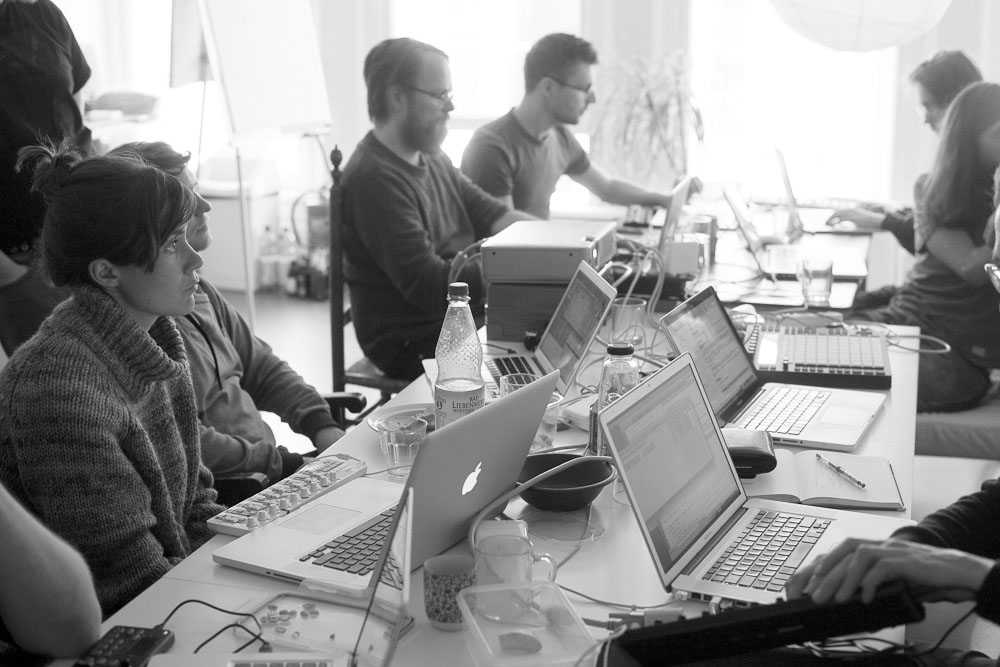
\includegraphics[width=.9\columnwidth]{../media/20140331-IMG_5976.jpg}
	\caption{Meeting 2014 at STEIM, Amsterdam.}
	\label{fig:media_20140331-IMG_5976}
\end{figure}

\section{Introduction}
\label{sec:introduction}

The \textit{Modality} project was initiated by Jeff Carey and Bj\o{}rnar Habbestad, who after several years of collaboration realised that, despite playing completely different setups, they both had the need to switch between functionalities easily while performing.  While both had custom implementations of this behaviour, it appeared to be not flexible enough, especially extending their setup felt cumbersome, original ideas got lost over the hassle of implementation of mapping rules.

Out of these observations arose the idea to gather a group of experts in sound and music computing (and specifically from the SuperCollider community) which eventually formed the ModalityTeam.
Beginning with five people, over the meetings, more people became involved, such that the group currently consists of 12 members.

The intention of this paper is two-fold:
After an introduction on the concept of modality and related work (Section~\ref{sec:modal_control}), it gives insight on work in an interdisciplinary team of loose collaboration, driven mostly by a shared interest in, on the one hand, sound, music, performance practice and software design and development on the other (Section \ref{sec:the_modality_meetings}).
Secondly, it reports on the outcomes in both conceptual and concrete implementation details (Sections \ref{sec:implementation} and \ref{sec:islands_and_bridges_uniform_protocols}).
The paper concludes with a reflection on the work done over the course of the last 5 years.

\section{The modality way}
\label{sec:modal_control}

The Modality project is dedicated to modal interaction with synthesis processes for physical control in performance and musical practice.
The name \emph{Modality} arose from the idea to investigate the creation and extensive use of modal interfaces.
One particular strength of such modal interfaces is that they allow fast changes and therefore a braoder variety for sonic discovery.
This can be of benefit when, for example, improvising with musicians playing acoustic instruments.
Out of this arouse the question on how HCI interfaces can be both conceptualised and actually built, in which a small set of physical controls are used for a relatively a amount of purposes.
We contend that integration of such on-the-fly remapping features helps to create flexible instruments that are powerful yet interesting and therefore rewarding to play and listen to. 

The primary product of the Modality project is the \emph{Modality Toolkit}, a software library that facilitates (a) access to hardware and software controllers, (b) flexible routing of control messages to generative processes, and (c) recording, filtering and further processing of controller signals.
The ModalityTeam, an international and transdisciplinary group of people that see themselves as users and developers for SC meets at regular intervals to work on the library, discuss issues around music performance and composition, and perform in self-organised concerts.

Modality, however, can also be understood as a social descriptor for the ModalityTeam.
The fact that a number of programmers and artists from different (music)cultures and nationalies meet up on a more or less regular basis does not necessarily imply that they share the same  understanding, let alone opinion.
It turned out that themes as fundamental to the Modality project as ``performance practice'', ``control strategies'' and even ``software paradigms'' were highly ambiguous and recognised in different ways.

Further, it turned out to be a learning process to not only hear other opinions but to also take them into account during software design and implementation.

As a third interpretation level of the term Modality serves the structure of the meetings.
Reflecting the divergence between participants, most of the meetings consisted of a broad spectrum of activities, namely developer phases in which the Modality Toolkit was implemented, public workshops disseminating knowledge about the Modality Toolkit, and concerts in which participants performed with their custom instruments.

To illustrate the process, the next section is a report on the modality meetings and their outcomes, combined with subjective analyses of the participants on the working process.



\subsection{Related work}
\label{sec:related_work}

%\todo{only mentions the multiton classes. it is a good idea to add a sentence that they are built upon unnamed XXFunc classes.}
%\todo{whay are the multiton classes here? could also be a note in implementation section.}

The Modality Toolkit stands in the tradition of a line of related systems, dedicated to control data flow and filtering.
Particularly, it is informed by systems like \emph{OSCulator}~\cite{troillard2012-osc}, STEIM's \emph{junXion}~\cite{-jun}, the \emph{Digital Orchestra Kit}~\cite{malloch2008-a-n} and SC's own \emph{multiton pattern} implementations.

% simple to complex
\begin{description}
	\item[OSCulator] 
		\enquote{[\dots] is the missing link between your controllers and your music or video software.}
		Assign events to messages
		Define operation ranges(for floats)
		Define different events to specific values (ints) 
	\item[junXion] 
		is a \enquote{[\dots] data routing application that can process [hardware] 'sensors' [\dots] using conditional processing and remapping}~\cite{-jun}. 
		It is a stand-alone program to be put in the middle between the control input layer and the synthesis layer.
The roots of its development lay in the advanced sensor input and data manipulation features of pioneering live sampling software LiSa [2]. 
LiSa's sampling engine is not further developed, as many software synths are available now to replace its functionality. 
Similarly, STEIM's groundbreaking sensor and interfacing technologies have now become readily available through a host of affordable controllers and DIY-kits, e.g.those based around the Arduino platform.

In JunXion, data flow is organized in Patches with an Input-Action-Output logic. 
Inputs can come from 8 different types of data sources, namely MIDI, HID, OSC, Wii Remote, Serial (Arduino et al), internal timers, and data derived from audio (amplitude- and pitch-tracking) and video (blob tracking). 
The Actions process data based on the input and a host of definable behaviors (switching, toggling, differentiation, integration, activity measurement) and conditions that can imply data from other sensors or values stored in variables and tables. 
Output can be generated as MIDI messages of many kinds, OSC messages, emulated mouse or keyboard events, Arduino and Wii Remote messages, and state change internal to JunXion, such as switching to a new bank of controller mappings. 

  \item[Digital Orchestra Toolkit] The Digital Orchestra Toolkit \cite{-dot} was created by McGill as part of the Digital Orchestra project, around \enquote{[\dots] a number of paradigms for the design, creation and performance of digital musical instruments in the context of a long-term interdisciplinary, collaborative environment. Issues related to mapping strategies, notation, the relationship of physical and musical gestures, robustness, responsiveness, and haptic feedback arose during the course of the project.}\cite{ferguson-2009}. The toolkit consists of a number of Max objects implementing various data processing units, as well as accessing various hardware devices or protocols.
	
	\item[Multiton design patterns in SC] 
		SuperCollider has flexible proxy objects for tasks, patterns, sound processes, and functions, which allow replacing the proxy's object while using it. (Modality follows these, e.g. in the |MKtl(<name>)| access scheme.)
		Named variants of these classes, like |Tdef|, |Pdef|, |Ndef|, or |MIDIdef|, |OSCdef| follow the multiton pattern by creating named instances only, and keeping them in a global dictionary. 
		Calling the constructor, e.g., |Ndef(\a)|, will find an existing instance by that name, or create it. 
		A second argument, |Ndef(\a, { LFSaw.ar })|, will replace the proxy's current object with the new one given. This is very useful in live coding situations, where remembering name/function pairs is much easier than doing full  variable administration by hand.
\end{description}


\begin{figure}[h]
	\centering
		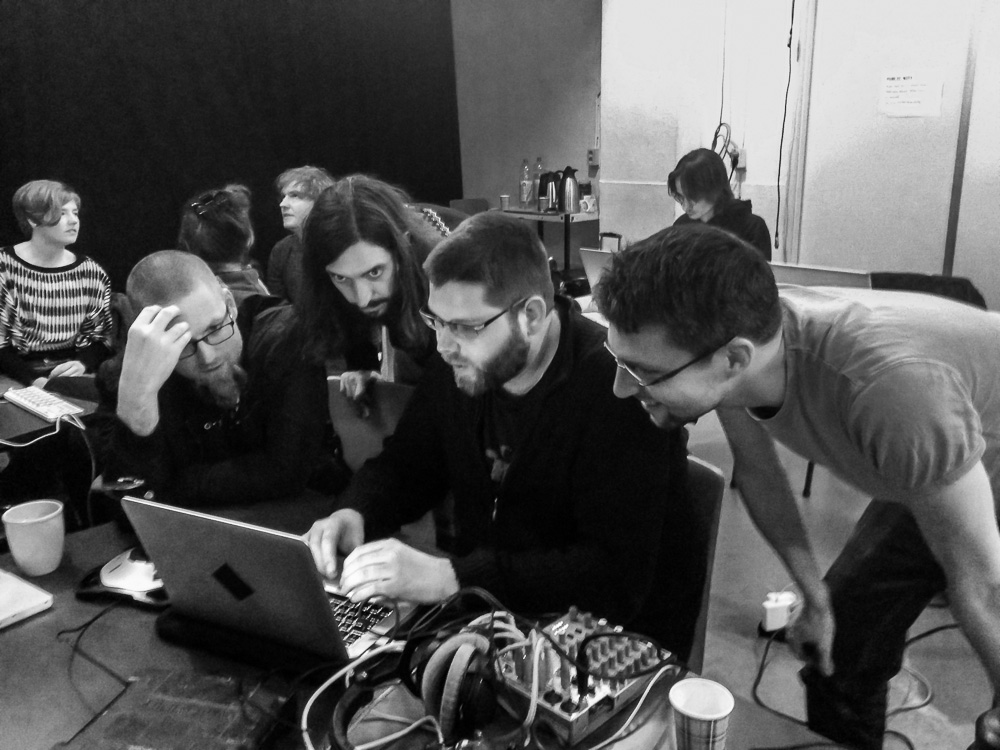
\includegraphics[width=.9\columnwidth]{../media/20140403-IMG_1667.jpg}
	\caption{Public workshop and open Lab at STEIM}
	\label{fig:media_20140403-IMG_1667}
\end{figure}




\section{The Modality meetings}
\label{sec:the_modality_meetings}

So far, the ModalityTeam held four meetings.

\begin{description}
	\item[October 2010, BEK, Bergen] Initiated by Jeff Carey and Bj\o{}rnar Habbestad, several experts and sound artists met to discuss shared ideas about modal control in performance and rehearsal situations.
	The attendees soon agreed that easy access and outlining of modal control structures is of great interest for all. First sketches for uniform access were made based on the then already existing JITMIDIKtl quark\footnote{a quark is an extension library in SuperCollider parlance.}, creating a more uniform access scheme to controllers in the Ktl quark. 
	
% 	\todo{add further description on founding meeting. Should be done by someone who actually was there.}
	
	\item[May 2011, STEIM, Amsterdam] Discussions revealed the need for users to abstract from hardware dependencies, and being able to do flexible routings and filtering incoming data. We therefore developed a new SC quark that began to implement two sets of functionalities:

|MKtl| objects for connecting to MIDI and HID hardware devices, and storing capabilities of each device in a configuration file. 
Instead of assigning functions to hardware-specifics, we considered controllers as a combination of \emph{controller elements}, which were given human-readable short names for semantically simple access, e.g. |'sl1'| instead of MIDI channel 0 cc 14.
This scheme was considered extensible for OpenSoundControl, serial ports, and other hardware interfaces, to have a uniform workflow, abstracted away from the actual backend.

|MDispatch| objects allowed creating \emph{calculation units}; abstract filters that render output from a given input, like the conversion of a button press (two states: on/off) to one trigger event (on), or the calculation of slider speed. Many templates for commonly used functionality were created.

A stumbling block at the time was the broken HID implementation in SC on OSX from version 3.5, due to changes in the API of Apple's HID toolkit. This has now been solved in version 3.7 with a new cross-platform HID implementation.

%	\begin{itemize}
%		\item |MKtl| objects for connecting to MIDI and HID hardware devices, and storing capabilities of each device in a configuration file.
%		 Instead of assigning functions to hardware-specifics 
%		 %like MIDI cc numbers, or an HID element cookies, 
%		 we considered controllers as a combination of \emph{controller elements}, 
%		 the |MKtlElements|, 
%		 which were given human-readable short names for semantically simple access, e.g. |'sl1'| instead of MIDI channel 0 cc 14.
%		 This scheme was considered extensible for OpenSoundControl, serial ports, and other hardware interfaces, to have a uniform workflow, abstracted away from the actual backend.
%		\item  |MDispatch| objects, which allowed creating \emph{calculation units}; abstract filters that render output from a given input, like the conversion of a button press (two states: on/off) to one trigger event (on), or the calculation of slider speed. Many templates for commonly used functionality were created.
%	\end{itemize}
%	
%	A stumbling block at this point was that the HID implementation in SC on OSX broke in the move to version 3.5, due to changes in the API of Apple's HID toolkit. This has only recently been solved in version 3.7 with a new cross-platform HID implementation.



	\item[November 2013, BEK, Bergen] After a hiatus of almost 2 years, this meeting focused on practical steps. 

	We created example use cases of different levels of complexity, in order to check how simple user code for these use cases can become, and to understand the concrete demands for the software better. 

We added unified functionality to the input layers: Explorers for MIDI and HID which listen to incoming messages from a source and can generate description files, and eventually responders for that source automagically. We also added hierarchical ordering of elements for more flexibility. 

Proposals for related useful concepts, such as FRP and Influx, were explored. Experimental items were moved outside the main toolkit.

	
%	\begin{itemize}
%		\item	We created example use cases of different levels of complexity, in order to check how simple user code for these use cases can become. 
%		\item 	We added unified functionality to the input layers: Explorers for MIDI and HID which listen to incoming messages from a source and can generate description files, and eventually responders for that source automagically. We also added hierarchical ordering of elements for more flexibility. 
%		\item 	Proposals for related useful concepts, such as FRP and Influx, were explored.
%		\item	Experimental items were moved outside the main toolkit.
%	\end{itemize}
		
%		\begin{itemize}
%		\item remove FRP
%		\item remove FuncChain
%		\item elementAt shortcut for getting element
%		\item sending values back to the device
%		\item MIDIExplorer
%		\item HIDExplorer
%		\item cleanup HID
%		\item Influx, Halo, DefLib as things to explore in Modality
%		\item Conform to the new description standard
%		\item added howto for description file generating. Lacks sections for HID and OSC.
%		\item implemented hierarchical specs
%		\item noteOn, noteOff, touch, cc work now, tested with MPD18.
%		\item move to VariousMixedThings
%		\item MIDIAnalysis more error checking
%	\end{itemize}
		
		
		
	\item[April 2014, STEIM, Amsterdam] 	Many aspects of the input side were unified and simplified further, thus nearing completion of the input layer.

Description file handling was improved in many ways, and fake GUIs can now be made for missing devices. Mapping strategies were simplified toward a unified style with |SoftSet|, |RelSet| etc. 

Much more documentation and examples were written, including more use cases sketched in text and written in some coding style variants.

Finally, HID in OSX was fixed, pending full tests.


%	\begin{itemize} 
%		\item HID support in OSX fixed (pending full tests)
%		\item Fake GUIs can now be made for missing devices
%		\item description file handling improved in many ways
%		\item Mapping simplified with SoftSet and RelSet
%		\item more use cases were sketched and written in some coding style variants
%		\item much more documentation and examples
%	\end{itemize}

%	\begin{itemize} 
%		\item Documentation updates
%		\item HID fix
%		\item adding MKtlGUI
%		\item hierarchical descriptions
%		\item add new SoftSet class and help file. will replace .softSet methods for several objects.
%		\item MIDIMKtl implemented polytouch and bend
%		\item refactoring device description loading
%		\item fake an MKtl
%		\item added SetRel command class for relative controllers.
%		\item cleanup of MKtl, allow using MKtl directly instead of MIDIMKtl, add infoMessage posting
%		\item Update description file reference to use Augmented Backus–Naur Form
%	\end{itemize}
\end{description}


\section{Islands, Bridges, uniform schemes}
\label{sec:islands_and_bridges_uniform_protocols}
As many home towns of modality members are harbor cities, Islands and Bridges were chosen as a mental model for conceiving and understanding highly modal instruments.
Islands are software objects or processes which represent sources (input devices, control-generating processes), destinations (output processes for sound, visuals), combinations of these, such as transformers (which, like destinations, process incoming control information, and send the results on like sources). 
Islands should be as self-sufficient as possible, and show uniform behavior to allow simple on-the-fly changes of connections with bridges. 

Bridges typically are made by user code that connects islands; conventional digital instruments then contain of a fixed collection of islands and one constellation of bridges between them. Modal performance instruments achieve their modes by switching between different combinations of bridges, adding some, removing others, adjusting settings. 
Modality aims to make writing and configuring bridges as simple as possible. 

In other words, Modality shifts the instrument metaphor from linear chains of command to flexible networks of communication (or further on, of mutual influence).

The uniform communication schemes recommended by Modality are largely based on existing conventions in SC, and extend them with only few new methods. Thus many SC quarks dealing with interface devices or data processing are useful sources for more islands. 
Beside the modality-toolkit\cite{githubmodality}, team actively work on many modality-relevant quarks: SenseWorld (supporting sensor devices), Manta (a controller), FPLib (containing FRP), VariousMixedThings (which includes Influx), UnitLib (?), wslib (many GUI-related niceties), KeyPlayer (contains KtlLoop), DMX (output to light systems), and others.

\subsection{ Uniform input device schema (MIDI, HID, OSC, GUI, Serial) }

Input devices (such as the |MKtl| class) or other control sources follow a scheme: 
They have rich descriptions, with simple short human-readable element names, which are hierarchically ordered where applicable. 
One can access each element by name or hierarchical name.
Each element can either have a single action, or one can add and remove multiple actions individually by identity or name.

Every |MKtl| can be replaced with a FakeGUI, which is made from its description file, and can generate all its control messages instead of the physical device.

\emph{Explorers} simplify adding new devices or sources: 
One activates every possible controller action at least once to collect specimens of every possible message type. 
Then an Explorer can make a description file template from this, and the user adds the final touches by giving them simple, short and clear element names, and organizing their hierarchical order. 
This is implemented fully for MIDI and HID, with other protocols to follow.

Transformer islands expect control input from sources, and know how to create control output for destinations. E.g. an |Influx| is a transformer which accepts m bipolar parameters from a source, and converts them to n process parameters for a destination with vectors of weights. 

\subsection{Proposed uniform destination schema}

%\todo{ miguel: I'm a bit skeptical about us really having a uniform protocol for destinations. MKtl allows registering call-backs for actions, so does Influx, etc, ok, but so do the stock SC guis, MIDIFunc, etc.  I wonder if we are not claiming too much by saying we have created uniform protocols when all that we are doing is providing call-backs which are known and used everywhere in SC. One could argue all of SC uses a uniform protocol which is calling methods on objects. Maybe I'm missing something here.
%}
%\todo{Till: I think, we should not claim to have a unified protocol for now. But maybe we can talk about the difficulties to get it up...}
% 
%\todo{adc: agreed, protocol is too big a claim. Maybe Proposed schema is the better term. below a short write-up, hope you find that useable?}

Modality-compatible sources have containers for configurable actions for sending messages to destinations, and they know how to convert their controller ranges to unipolar.

Modality-compatible destinations also follow existing SC schemes: They respond to set messages for control values; they remember current parameter values, and they often have specifications for control parameters (i.e. range, warp, step size, etc). Most objects that are active processes respond to .play, .stop, .pause and resume messages. 

Requiring destinations to know their parameters specs and current states allows more flexible control in several ways: 
The |setUni| method can be used to set a param from the controller side's unipolar value; keeping the spec with the destination process is semantically simpler, and multiple control sources will immediately use changed specs if they belong to the object. 
The |RelSet| class method can be used to nudge a parameter relative to its current value. 
|SoftSet| class methods can be used to take over a parameter only when the physical controller is close enough to its value, or when the physical controller knows the object's previous value well enough (which is the case when it has set it to that value). 
If specs are kept with the object, they can easily be adjusted there (e.g. for zooming into a subset of the full range), keeping the controller element side code simpler by sending unipolar values, and letting the object provide the spec:

|{ arg el; dest.setUni(\amp, el.value) }|

Finally, conforming to the SC convention of |play/stop|, |pause/resume| allows very simple de/activation when switching newly to or away from a process. 

\section{Examples / Use Cases}
\label{sec:examples_use_cases}

We created a number of simple to medium-complex uses cases, which serve both as examples for modality concepts, and as test cases that show how simple they can be implemented in different coding styles. 

\subsection{MPD 18, copy sounds between locations}
\label{sub:mpd_18}

The Akai MPD18 controller has 16 Buttons and a slider. In this use case, the buttons correspond to locations where sound processes can be. When a sound is active, the slider controls one of its parameters. sounds can be copied between locations.

\begin{description}
 \item [Sound Buttons] Buttons 1-3 are mapped to adsr enveloped sound sources.
        By pushing them down, the sound turns on; upon releasing, the sound decays.
    the slider sets amplitude (or pitch) for the (sound)source of the currently depressed button.
 \item [Memory Slots] Buttons 5-16 represent 'memory' positions (initially not mapped)
        if sound is assigned (see below), sound is played when button depressed.
 \item [Shift Button] Button 4 is a 'shift key'. When depressed
        Sound Buttons don't trigger any sound but select the active slot. This can be followed by
        depressing a Memory Slot button, which assigns the selected sound to that pad.
        if you release the shift key before assignment, nothing happens.
        assigning a copy to an already assigned memory slot replaces existing
        mute copy + [Sound Button then Shift button]
        Sound Button triggers sound
        depress Memory Slot button, assigning the sound to the pad, with sound
\end{description}
       
\subsection{Switching actions}
\label{sub:switching_actions}

Switching actions from one controller to another mid-way through a performance.

\subsection{An example of a performance setup with Influx and KtlLoop}

\emph{Would this make sense here ?}



\section{Specification, design and implementation of the Modality toolkit}
\label{sec:implementation}

\subsection{Specification}
\label{sub:specification}

% taken from the workshop webpage. please adjust/remove/edit.
The Modality toolkit aims to facilitate
\begin{itemize}
	\item data acquisition from commercially available controllers (e.g. HID and MIDI) by providing a common software interface,
	\item processing of control data streams,
	\item sending control data to these controllers (e.g. fader positions, LED states),
	\item graphical feedback  of the current state in the form of a GUI of connected a device, as well as replacing a controller with a GUI substitute, and finally
	\item mapping the output of these data streams to input parameters of sound engines.
\end{itemize}

Specific attention is given to the concept of modal control: the ability to change the mapping on-the-fly from one control element to another, possibly located on another device.
Or to change assigned functionality of one control element based on the state of another, as in changing the function of an alphanumerical key by using the SHIFT key on a computer keyboard.
% %%%%%%%

\subsection{Implementation}
\label{sub:implementation}

The Modality Toolkit is implemented as a set of classes for the SuperCollider language \cite{mccartney2002-ret}. 
The control elements of devices are accessed through the |MKtl| class. 
A control element is a part of a controller that either generates and/or accepts a one-dimensional stream of events. 
Each |MKtl| object consists of elements such as sliders, knobs, buttons or encoders.
It is possible to assign actions to such elements that are evaluated every time the value of that element gets updated.
Elements are instances of |MKtlElement| and are kept in a tree-like data structure using nested arrays and dictionaries which represents the spatial grouping of control elements in the physical controller. 
For convenience, elements can also be accessed from a flat array using the |allElement| method. 
The |elementDescription| variable of MKtlElement contains a dictionary with information about that element such as it's type (e.g., button, slider) and control spec for scaling incoming values. 
This dictionary can be used to extract multiple elements from the data structure by filtering using a conditional expression, for instance retrieving all elements of type |slider|.

Using the multiton pattern described in Section~\ref{sec:related_work}, each |MKtl| has a name, and only one |MKtl| is active with that name at any given time. 
MKtl's can be retrieved from a global dictionary by name, using the |MKtl('name')| syntax. 
The system keeps a global set of auto-generated names for all the controllers that have description files. These short names are auto-generated from the name of the device plus a number starting from zero indexing multiple identical devices (e.g. |'nnkn0'| from |'nanoKONTROL'|). If a user tries to fetch an MKtl with one of the auto-generated names and it is not yet created the system will look for the corresponding device and if it is found an MKtl is created from the description file and connected to the device by creating MIDI or HID responders. This feature means the user can initialize an MKtl for a given device using always the same single line of code.

\begin{Verbatim}
k = MKtl('nnkn20');
\end{Verbatim}

Actions are added to elements by setting the MKtlElements' |action| to a function. This function is called every time an event is received from that control and it is passed the MKtlElement instance. It's possible to add and remove multiple actions to the same element using the |addAction| and |removeAction| methods which use the |FunctionList| class. Optionally, one can use the FuncChain class where functions can be added and removed by name, as well as reordered, and flexibly enabled and disabled for switching between modes. 

\begin{Verbatim}
//add action
MKtl('nnkn20')
.elements[\sl][0]
.action = { |e|
  var freq = e.value
  .linlin(0.0,1.0,300,3000);
  x.set(\freq, freq)
};

//remove action
MKtl('nnkn20')
.elements[\sl][0]
.action = nil
\end{Verbatim}

Some elements (with |ioType| |'out'| or |'inout'|) can also send values back to the device, this is done using the |value_| method of |MKtlElement|.

\begin{Verbatim}	
MKtl('bcr20000')
.elements[\kn][0][0]
.value_(0.3)
\end{Verbatim}

\subsection{Unifications of interface implementations}
\label{sub:unifications_of_interface_implementations}

The Modality Toolkit works uniformly across multiple protocols. The base class MKtl provides the generic functionality and the children classes (|HIDMKtl|, |MIDIMktl|, |OSCMKtl|, etc.) implement the specific back-end for each protocol. Since the interface for using Modality is defined in |MKtl| and |MKtlElement|, which are protocol agnostic, the syntax and semantics remain uniform across all protocols. The incoming values from the device are normalized to be in the range $[0,1]$ and outgoing values are expected to be in $[0,1]$ range and then scaled to the range used by the specific protocol. This facilitates switching between devices that use different protocols while keeping the event logic unaltered.

MKtl also has the useful feature of automatically creating a GUI representation of a known device from it's description file. If the user tries to instantiate an MKtl with an auto-generated name corresponding to a known device, but the device is not currently available, an |MKtlGui| will be automatically created instead. This makes it trivial to exchange a physical controller for a GUI representation without having to change any code at all.

\subsection{Description files}
\label{sub:descriptions_files}

In order to use a device within the Modality Toolkit context, a \textit{device description} file is needed that characterises each control element and its semantical position in relation to other elements.
It is implemented using one text file per device containing a dictionary with the fields 
\begin{description}
	\item[protocol] currently, HID and MIDI are implemented. Note that only one protocol per device is allowed,
	\item[device] the name of the device as provided by the operating system,
	\item[description] a dictionary with a tree structure composed of nested dictionaries and arrays. The value at each leaf of the tree is an element dictionary with key-value pairs describing the element at hand.
	An element dictionary contains technical specifications of the element, namely identification information (e.g. for MIDI, the MIDI number and channel), the physical type of control (button, slider, etc.) and a |ControlSpec| that specifies how to convert the incoming values to the range $[0,1]$.
\end{description}

As an example, the element dictionary for a button of a MIDI device would look like this:
\begin{Verbatim}
\rew: (
	\midiMsgType: \cc,
	\type: \button,
	\midiChan: 0,
	\midiNum: 47,
	\spec: \midiBut,
	\mode: \push
)
\end{Verbatim}

Elements which are physically (or virtually) grouped on the device such as with pages, rows or columns are grouped together in the description file using arrays. For instance, the third button on the second row of page 4 of a Korg NanoKONTROL can be accessed with the following code, assuming zero-based numbering:

\begin{Verbatim}
MKtl('nnkn0').elements[\sl][3][1][2]
\end{Verbatim}

The hierarchical grouping of elements also facilitates bulk addressing of elements by traversing the hierarchy starting at the desired node. For instance, it's easy to programatically add actions to multiple elements:

\begin{Verbatim}
MKtl('nnkn0').elements[\sl]
.do{ |xs, page|
 xs.do{ |xs, row|
  xs.do{ |element, column|
   element.action = 
    {[page, row, column].postln}
  }
 }
}
\end{Verbatim}

The standard order for grouped elements is first page, then row starting from the top of controller and finally column starting from the left of the controller.

New devices can be added to modality easily, all that is needed is to write the corresponding device description file. 
If a user tries to access a device for which there is still no description file available, the toolkit guides the user in the process of creating the description file. 
More specifically, a description file can be generated for HID devices using the |HIDExplorer| class, which collects information provided by the low-level HID stack. 
For the less self-documenting range of devices connected via MIDI, the user is asked by the |MIDIexplorer| class to operate all available physical controls. 
The captured data stream is then used to generate a description file.
As a last step in both cases, the user supplies suitable labels and orders the elements hierarchically according to their physical placement on the device.




\begin{figure}[h]
	\centering
		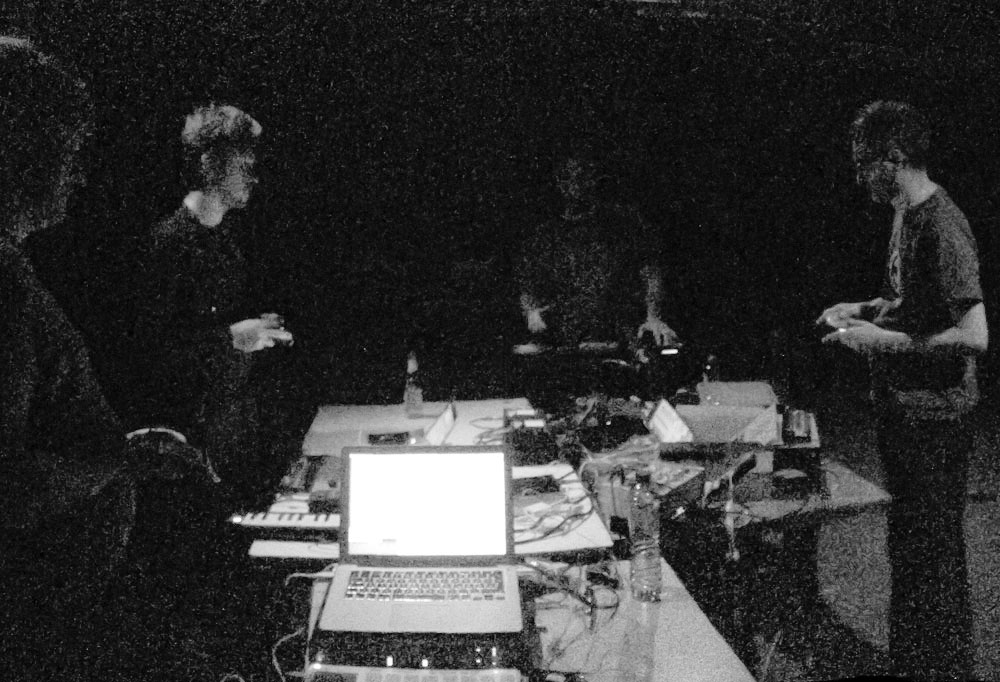
\includegraphics[width=.9\columnwidth]{../media/20140405-IMG_1691.jpg}
	\caption{Modality Concert 2014 at OT301}
	\label{fig:media_20140405-IMG_1691}
\end{figure}

\subsection{Modality related projects and quarks} 

\todo {Longer descriptions of MDispatch, FRP, Influx can go here.}


	
\subsubsection{MDispatch}	

The MDispatch class was an initial attempt at creating self-contained event logic units. |MDispatch| has similar structure as |MKtl| (both inheriting from |MAbstractKtl|). A dispatch has output elements (|MDispatchOut| class) where actions can be added similarly to |MKtlElement|. It also also has inputs which are updated by registering callbacks on the elements of other |MAbstractKtl|s. When an event is received from a source the input element and it's value are saved and a list of state processing functions is run sequentially. These state processing functions have access to all the internal state of the dispatch which includes the source element which caused the update, all the values of the output elements and any other state variables defined for auxiliary calculations. An MDispatch can be either created from a template containing predefined functionality or explicitly defined. The process for explicitly creating an MDispatch is to specify outputs, define state processing functions and finally connect the dispatch to sources of events. In order to facilitate this process it is possible to first connect to a source and just copy the output names of the source to the output names of dispatch, in fact mirroring the same elements. This makes it easy to create path-through processors which just take the output of each element of an MKtl and do some processing with it and then output a value through an element with same key. Below is the code for creating a dispatch that only outputs when incoming values are increasing and takes values from a midi device:

\begin{Verbatim}
k = MKtl('nnkn0');
d = MDispatch.make(\up, k);
\end{Verbatim}

At the time when MDispatch was created several templates were written for tasks such as for soft paging, getting velocity values or filtering events. 

MDispatch was an interesting experiment that allowed for some degree re-usability of event logic code, nevertheless it's interface was slightly cumbersome since it acted as a virtual device with many inputs and outputs, with explicit creation of outputs, registering for inputs and management of connections. Creating smaller and therefore more re-usable dispatches was discouraged by the burden of all the necessary initialization code. Perhaps because of these issues MDispatch did not gain wide adoption amongst users of the Modality toolkit and it's development is currently paused. \emph{ would be good to get other opinions on this. Do you agree with what I say in this paragraph ? }
		
\subsubsection{FRP}

\todo{functional) reactive programming: the icmc is full of people, who
use(d) pd/max, which has a reactive semantics. maybe a quick comment on
this may be helpful for many people of the intended audience}

An electronic instrument can be though of as set of inputs from control devices, a set of audio units or processes that create audio units and control logic in between to allow incoming events from the physical devices to affect the state of the audio units. 

The traditional method of dealing with incoming events is through callback functions. A callback function is registered and it is called every time an event is received. Callback functions, although easy to define lack composability and require all the basic patching to be handled by user. Functional Reactive Programming, or FRP, is a paradigm for programming dynamic and reactive systems using first-class composable abstractions that tries to address some of these issues. The two main abstractions are event streams (sequences of discrete-time event occurrences) and behaviours or signals (time-varying values). Most of the original work on FRP was done on the Haskell programming language\footnote{Haskell is a modern, pure, lazy, statically typed functional programming language.} with two main flavors, Classic FRP~\cite{elliott1997-fun,elliott2009-pus} and Arrowized FRP~\cite{hudak2003-arr,courtney2003yampa}.

The FRP paradigm seemed promising for the construction of musical digital instruments, so in order to make it available in the SuperCollider language the \emph{reactive-web} library from the Scala language was ported to SC and extended. Ideas from \emph{reactive-banana}, a modern FRP library for Haskell, were also incorporated. This SuperCollider FRP implementation is part of the FPLib library~\cite{-fpl} which makes available a number of functional programming constructs such as Monads and Applicative Functors in SC.
 
In FP-Lib, the main entities for FRP are the EventStream and FPSignal classes. Signals are slightly different from the behaviors of Classic FRP: behaviors model any continuous time function $f:Time\rightarrow A$, while signals only model step functions.  Outputs are defined in terms of inputs using \emph{combinators} (pure functions) applied to the signals or event streams in order to construct an \emph{event graph}. To get events into the event graph the system has to register with external sources, the inputs, and to have any effect on the outside world it must perform actions based on the outputs of the event graph. The \emph{event graph} together with \emph{inputs} and \emph{outputs} forms an \emph{event network}. To build an \emph{event network} the inputs, outputs and event graph are described in a definition which can then be compiled into a working event network. The compiled event network can be started and stopped at any moment, stopping it disconnects from all registered event sources and stops performing all output actions.

It's possible to create complex programs with time\\-dependent logic by composing  event streams and signals using a small set of combinators:

\begin{itemize}

\item transforming event streams into signals and vice-versa:
\begin{Verbatim}
sig1 = es1.hold(0.0)
es2 = sig2.changes
\end{Verbatim}
\item Merging multiple event streams into one event stream by accepting events from any streams:
\begin{Verbatim}
mergedEs = es1 | es2 | es3 | es4
\end{Verbatim}
\item Filtering events of an event stream using a function that returns a boolean:
\begin{Verbatim}
es.filter({ |x| x > 0.5 })
\end{Verbatim}
\item Keeping state that can be influenced by several different event streams by  associating each event stream with a state altering function. The state is first set to an initial value, then each time the event streams receive an event it generates a new function to be applied to the current value of the state. For example, a counter that can be incremented by one event stream and decremented with another:
\begin{Verbatim}
( es1.collect{{|x|x+1}} | 
  es2.collect{{|x|x-1}} )
.injectF(0) 
\end{Verbatim}
\item Merging n signals using an n-ary function. This is possible to do with signals but not with event streams, since only signals remember their last value. For example, converting two signals carrying x and y coordinates to one signal carrying the angle: 
\begin{Verbatim}
atah2(_,_).lift.(xSig, ySig)
\end{Verbatim}
\item Applying a time-varying function (stored in an signal) to an event stream. This allows event streams to use previous values from other nodes in the graph. For example, starting a synth on pressing a pad with frequency determined by the last value of a slider:
\begin{Verbatim}
{ |f,e| IO{Synth(\a,[\freq,f])} }
<$> sliderSig <@> padEs 
\end{Verbatim}
%$ need this otherwise texmaker turns all my text to green
\item Dynamic event switching: changing the event graph by running a function on an incoming event that returns the new event stream or signal to use. For example, every time a signal emits an int $n$, create a new signal that merges the first $n$ elements of a list of signals using an averaging function: 
\begin{Verbatim}
sigNum.switchInto{ |n|
  listOfSignals[..n].sequence
  .collect{ |xs| xs.sum / xs.size }
}
\end{Verbatim}
All FRP objects created inside the function are automatically disposed off when the function is run again preventing leaks.
\end{itemize}

In FP-Lib, inputs to the event graph can come from MIDI or HID (via the
Modality Toolkit), OSC, GUIs or Timers and are declared using  the |enIn| (signal) or |enInES| (event stream) method. Outputs are declared by calling |enOut| on a signal or event stream that carries actions to be performed (elements of the IO monad, which in SC are anonymous functions wrapped in a class). For convenience there are predefined actions available called \textit{sinks}. Passing an FRP object to a sink will execute the default action of the sink using the values emitted by the object.

FPLib can be used in conjunction with UnitLib, in which case the definition of the event network should return a dictionary of synth control names to Signals or event streams. The output of the frp objects can then be automatically scaled to the range of the parameter of the synth, since units have a control spec for each control in the SynthDef.

Since all the functions used to construct the graph are pure\footnote{SuperCollider is not a typed pure FP language like Haskell, so there are no guarantees that the functions passed by the user to the to the FRP combinators are actually pure, it's up to the user to make sure that this is the case.} it's possible to abstract a subset of them into a single function and be confident that the result will be identical. Also, the event graph does noy depend on the nature of the inputs or outputs, for instance MIDI inputs can be changed to GUIs or OSC messages without changing any of the event graph code. This makes it easy to build a personal library of event logic functions that can be re-used for different instruments or different parts of the same instrument.

Several use cases put forward by the Modality Team have been implemented using FPLib and so far the system as shown itself capable of creating complex event graphs to be used in digital instruments. The FRP system has not gained wide adoption amongst Modality users either, perhaps because pure functional programming is quite a different paradigm from the imperative object\\-oriented paradigm of SC.

\subsubsection{Influx}

describe

\subsubsection{others}

which ones ? SenseWorld, 


\section{Conclusions}
\label{sec:conclusions}


Claims to originality:
* incoming data is associated with a rich knowledge of what generated it. possible to query elements based on type.
* access to elements done in a logical and easy-to-remember way, both through the auto-generated device names and element hierarchy.
* automatic initialization reduces startup to one line of code.
* Uniform access to controls from devices across multiple controllers and protocols.
* Several ways to take inputs and create complex instruments investigated.

* Modality takes the strongest
We have showed beyond doubt that Modality is the best thing since sliced bread. It surpasses all other solutions out there both already invented and to be invented in the future. Resistance is futile, you will modalidated.


\begin{acknowledgments}
The Modality team is (in alphabetical order):
    Marije Baalman,
    Tim Blechmann,
    Till Bovermann,
    Alberto de Campo,
    Jeff Carey,
    Bj\o{}rnar Habbestad,
    Dominik Hildebrand Marques Lopes,
    Amelie Hinrichsen,
    Robert van Heumen,
    Hannes Hoelzl,
    Miguel Negr\~{a}o, and
    Wouter Snoei.
Associated organisations are (in alphabetical order):
BEK,
the project \emph{Design, Development and Dissemination of New Musical Instruments} of UdK Berlin/TU Berlin, supported by the Einstein Foundation,
nescivi, and
STEIM.

The Modality meetings have been funded by Bergen Kommune, Nordisk Kulturfond and Creative Industries Fund NL.


\end{acknowledgments} 

%%%%%%%%%%%%%%%%%%%%%%%%%%%%%%%%%%%%%%%%%%%%%%%%%%%%%%%%%%%%%%%%%%%%%%%%%%%%%
%bibliography here
\bibliography{icmcmodality}

\end{document}
